

\section{Introduction}

A robot is an actor in its environment and not simply a passive
observer.  This gives it the potential to examine the world using
causality, by performing probing actions and learning from the
response.  Tracing chains of causality from motor action to perception
(and back again) is important both to understand how the brain deals
with sensorimotor coordination and to implement those same functions
in an artificial system, such as a humanoid robot.

\ifverbose
In the context of sensorimotor coordination causality can be operationally
defined as a functional link between some variables, being these motor,
sensorial, or both.  At higher levels of abstaction other quantities might
need to be considered, not necessarily, purely sensorial or motor but
rather combinations of various sort. Causality accounts to discovering
similarity and recurrence in this sensorimotor data, possibly delayed of
unknown amounts.
\fi

In this paper, we propose that such causal probing can be arranged in
a developmental sequence leading to a manipulation-driven
representation of objects.  We present results for two important
steps along the way, and describe how we plan to proceed.

Table~\ref{tab:causation} shows three levels of causal complexity.
The simplest causal chain that the robot experiences is the
perception of its own actions.  The temporal aspect is immediate:
visual information is tightly synchronized to motor commands.
We use this strong correlation to identify parts of the robot
body -- specifically, the end-point of the arm. 

Once this causal connection is established, we can go further and use
it to active explore the boundaries of objects.  In this case, there
is one more step in the causal chain, and the temporal nature of
the response may be delayed since initiating a reaching movement doesn't
immediately elicit consequences in the environment.  

\ifverbose
relation and a
more subtle perception of space has also to be taken into account, e.g
localization of the effector, and the spatial relation with the
manipulated object.  The temporal aspect in this case assumes a
delayed form: triggering a reaching movement doesn't immediately
elicit consequences in the environment.


We
show how an active exploration strategy might explain how newborns
develop, during ontogenesis, figure-ground segregation capabilities.
The temporal aspect in this case assumes a delayed form: triggering a
reaching movement doesn't automatically elicit consequences in the
environment. Towards reaching completion a more immediate form can
take place due to correlation between the haptic and visual responses.
\fi

Finally we argue that extending this causal chain further will allow
us to approach the representational power of ``mirror
neurons''~\cite{fadiga00visuomotor}, where a connection is made
between our own actions and the actions of another.

\ifverbose
The third case is a more conceptual one and it represents our more long
term goal in terms of robotic implementation. It is interesting though
because it can be explained by the same principle of causality. This
is the case of ``mirror neurons''~\cite{fadiga00visuomotor}. The
details of this third example are presented later.  Development takes
an even more delayed form involving probably a form of long-term
memory. Our everyday personal experience on the manipulation of objects is
reused to interpret the same class of manipulative acts when performed
by somebody else.  Clearly the two situations, when acting and when watching,
 are not necessarily simultaneous.
\fi

\ifverbose
This solves a problem,
difficult if addressed visually, by taking advantage of the fact the
system is embodied.  There are examples of similar behaviors in
newborns [I still have to find the refs in this case]. The level of
causality exploited here is a direct one. 
\fi

\ifverbose
  Of
course, processing delays must be accounted for -- in the brain,
delays are known to depend on the modality (e.g. vision is slower than
for example vestibular signals) and consequently multisensory or
sensorimotor integration has to compensate for them.
\fi



\ifverbose
There is a bulk of neuroscience data on all this aspect of human
sensorimotor cognition. For the purpose of this paper, we first would
like to show that there is indeed a problem if the agent is not
properly situated[? does it make any sense ?]. A nice example is the
definition of ``object''.  We will devote a
section to illustrate this point which turns out to be central in a
series of tasks including the three cases analyzed before. Many of our everyday's
acts are definitely object-oriented.

Developmentally we can explain what is an ``object'' by exploiting
the fact that the agent is embodied.
By looking at the three examples, we can notice a trend in complexity, 
and consequently we can hypothesize, that the time required to reach proficiency 
in each task is proportional to this complexity. Table~\ref{tab:causation} shows this idea.
\fi

\begin{table*}[htbp]
\begin{center}
\begin{tabular}{|p{4.8cm}|p{4.8cm}|p{4.8cm}|}
\hline
{\it type} & {\it nature of causation} &  {\it time profile} \\ \hline\hline
{\bf sensorimotor coordination} & direct causal chain & strict synchrony \\ \hline
{\bf object probing} & one level of indirection & fast onset upon contact, potential for delayed effects\\ \hline
{\bf mirror representation} &  complex causation involving multiple causal chains & arbitrarily delayed onset and effects\\ \hline
\end{tabular}
\caption{
\label{tab:causation}
%
Degrees of causal indirection. There is a natural
trend from simpler to more complicated tasks.  The more time-delayed
an effect, the more difficult it is to model.
%
}
\end{center}
\end{table*}



\ifverbose
The more strict
temporal aspect on the other hand require perfect timing (within the
bandwidth of the process considered of course), but the cause-effect
linkage is a direct one.
For the purposes of manipulation, we would like to know what parts of
the environment are physically coherent ensembles -- that is, which
parts will move together, and which are more or less independent.  It
takes a great deal of experience before this judgement can be made
from purely visual information.  This paper develops active strategies
for acquiring that experience through experimental manipulation, using
tight correlations between arm motion and optic flow to detect both
the arm itself and the boundaries of objects with which it comes into
contact.
\fi

\section{The elusive object}

\label{sect:introduction}

Sensory information is intrinsically ambiguous, and very distant from
the world of well-defined objects in which humans believe they live.  
What criterion should be applied to distinguish one object from
another?  How can perception support such a phenomenon as figure-ground
segmentation?  
Consider the example in Figure~\ref{fig:number-cross}.  It is
immediately clear that the drawing on the left is a cross, perhaps
because we already have a criterion, which allows segmenting on the
basis of the intensity difference. It is slightly less clear that the
zeros and ones on the middle panel are still a cross. What can we say
about the array on the right? If we are not told, and we do not have
the criterion to perform the figure-ground segmentation, we might
think this is just a random collection of numbers. But if we are told
that the criterion is ``prime numbers vs. non-prime'' then a cross can
still be identified.

While we have to be inventive to come up with a segmentation problem
that tests a human, we don't have to go far at all to find something
that baffles our robots.  Figure~\ref{fig:setup-sequence} shows a
robot's-eye view of a cube sitting on a table.  Simple enough, but
many rules of thumb used in segmentation fail in this particular case.
And even an experienced human observer, diagnosing the cube as a
separate object based on its shadow and subtle differences in the
surface texture of the cube and table, could in fact be mistaken --
perhaps some malicious researcher is up to mischief.  The only way to
find out for sure is to take action, and start poking and prodding.
As early as 1734, Berkeley observed that:
%
\begin{quote}
...objects can only be known by
touch. Vision is subject to illusions, which arise from the
distance-size problem... \cite{berkeley72new}
\end{quote}
%
In this paper, we provide support for a more nuanced proposition: that
in the presence of touch, vision becomes more powerful, and many of
its illusions fade away.


%
\begin{figure}[tb]
\begin{center}
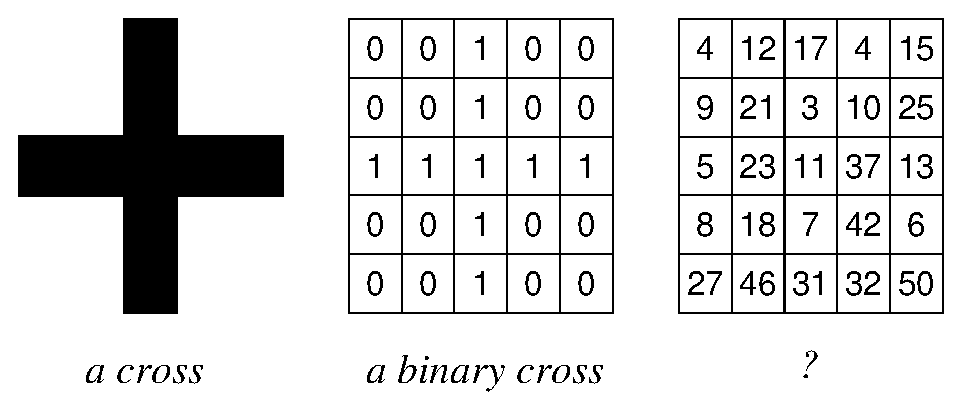
\includegraphics[width=6.5cm]{number-cross.eps}
\caption{ 
\label{fig:number-cross}
%
Three examples of crosses, following~\cite{manzotti01coscienza}.  The
human ability to segment objects is not general-purpose, and improves
with experience.
%
}
\end{center}
\end{figure}
%
%
\begin{figure}[tb]
\begin{center}
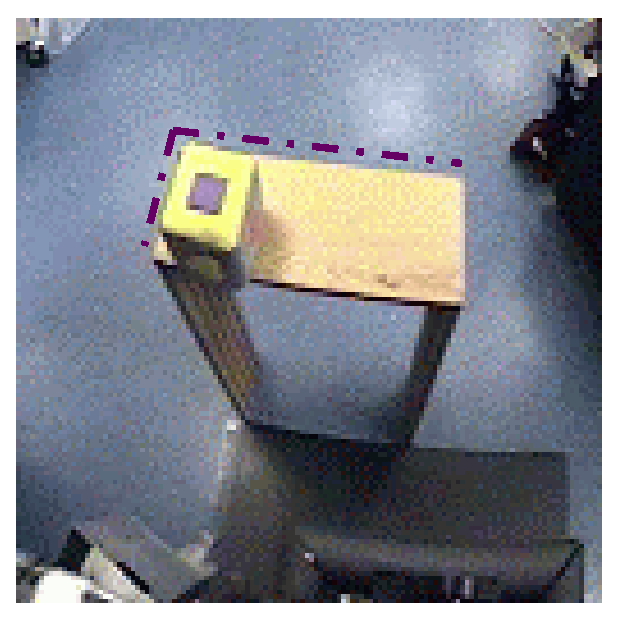
\includegraphics[width=4cm]{setup-sequence.eps}
%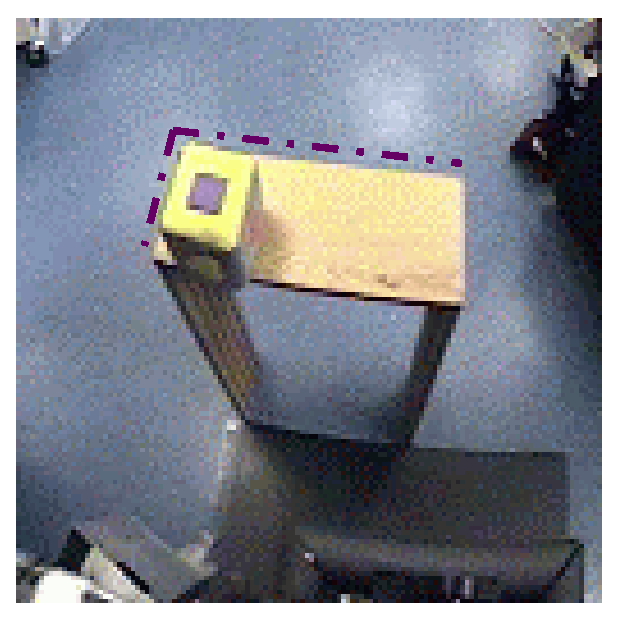
\includegraphics[width=\columnwidth]{setup-sequence.eps}
%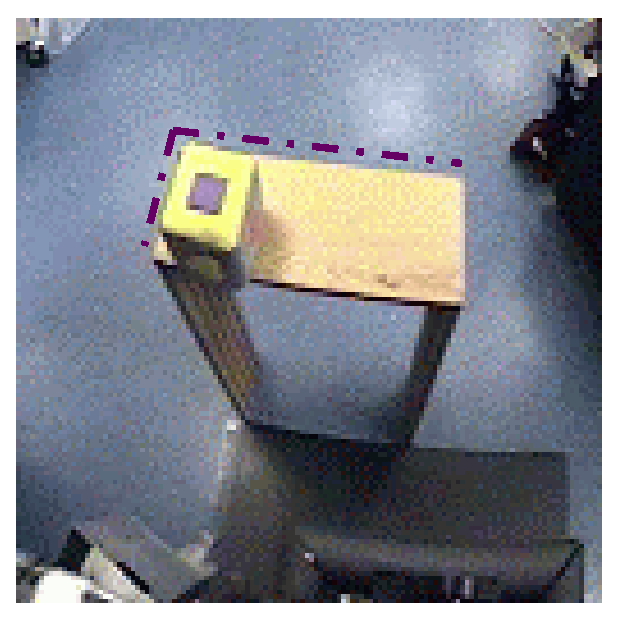
\psfig{file=setup-sequence.eps,width=4cm}
\caption{ 
\label{fig:setup-sequence}
%
A cube on a table. The edges of the table and cube happen to be
aligned (dashed line), the colors of the cube and table are not well
separated, and the cube has a potentially confusing surface pattern.
%
}
\end{center}
\end{figure}

%
%
%
\subsubsection*{Objects and actions}

The example of the cross composed of prime numbers is a novel (albeit
unlikely) type of segmentation in our experience as adult humans.  We
might imagine that when we were very young, we had to initially form a
set of such criteria to solve the object identification/segmentation
problem in more mundane circumstances.  That such abilities develop
and are not completely innate is suggested by results in neural
science. For example Kovacs \cite{kovacs00human} has shown that
perceptual grouping is slow to develop and continues
to improve well beyond early
childhood (14 years). Long-range contour integration was tested and
this work elucidated how this ability develops to enable extended
spatial grouping.  

\ifverbose
The pattern of interconnections in the visual cortex is also known
to complete development postnatally from cell staining methods
studies~\cite{burkhalter93development,callaway92development}.
Brown~\cite{brown94vision} argued that a developmental process, that
is one of structure formation, is involved in acquiring visual
abilities rather than a pure parameter adaptation procedure as in
machine learning algorithm.
\fi

Key to understanding how such capabilities could develop is the
well-known result by Ungerleider and Mishkin \cite{ungerleider82two}
who first formulated the hypothesis that objects are represented
differently during action than they are for a purely perceptual task.
Briefly, they argue that the brain's visual pathways split into two
main streams: the dorsal and the ventral~\cite{milner95visual}. The
dorsal deals with the information required for action, while the
ventral is important for more cognitive tasks such as maintaining an
object's identity and constancy.  Although the dorsal/ventral
segregation is emphasized by many commentators, it is significant that
there is a great deal of cross talk between the streams.  Observation
of agnosic patients \cite{jeannerod97cognitive} shows a much more
complicated relationship than the simple dorsal/ventral dichotomy
would suggest.  For example, although some patients could not grasp
generic objects (e.g.  cylinders), they could correctly preshape the
hand to grasp known objects (e.g. a lipstick): interpreted in terms of
the two pathways, this implies that the ventral representation of the
object can supply the dorsal stream with size information.

%[Might need to add a picture to explain the connections]


Grossly simplifying, the brain circuitry responsible 
for object oriented actions is thought to consist of at least four 
interacting regions: the primary motor cortex(F1), the premotor cortex (F4, F5), the 
inferior parietal lobule (AIP, LIP), and the temporal cortex 
dealing with the semantic content of the action 
(TE, TEO) (\cite{rizzolatti-fogassi-gallese-1997}\cite{fadiga00visuomotor} 
for a review). While this is a useful subdivision, it is worth to bear in mind 
that the connectivity of the brain is much more complex, that bidirectional 
connection are present, and that the resulting behavior is the result of a 
population activity of these areas. The example about the grasping of known 
objects in agnosic patients testifies the abundance of anatomical connections 
between different regions.

Another way of looking at the same connectivity is in terms of the main 
function of each area. For example F4 and LIP are involved in the control of 
reaching, F5 and AIP contain the majority of grasp related neurons, 
and TE, TEO are thought to subserve object recognition. They form a network 
of parallel and yet interacting processes. In fact, at the behavioral level, it has 
been observed \cite{jeannerod-arbib-rizzolatti-sakata-1995} that reaching and 
grasping need to interact to correctly orient and preshape the hand.

Reaching responsive neurons are present in the inferior parietal lobule. For 
example, Jeannerod et al. \cite{jeannerod-arbib-rizzolatti-sakata-1995} reported 
that the temporary deactivation of the caudal part (VIP) - by injecting a GABA 
agonist - of the intraparietal sulcus 
disrupts reaching. Conversely, injection in the more rostral part (area AIP) interferes with 
preshaping. Some of the VIP neurons have bimodal visual and somatic receptive 
fields (RF). About 30\% of them have a RF which does not vary with 
movement of the head \cite{rizzolatti-fogassi-gallese-1997}. The tactile and 
visual RF often overlap (e.g. a central visual 
RF corresponds to a tactile RF in the nose or mouth). The parietal cortex contains 
also cells related to eye position/movements that are likely to be involved into 
the visuo-motor transformation required for reaching. VIP projects to area 
F4 in the premotor cortex. Area F4 contains neurons that respond to objects and 
are related to the description of the peripersonal space with respect to reaching 
\cite{graziano-hu-gross-1997}\cite{fogassi96coding}. A subset of the F4 neurons 
has a somatosensory, visual, and motor receptive field. The visual receptive 
field extends in 3D from a given body part, for example, the forearm. The somatosensory RF
is usually in register with the visual one. Finally, motor information
is integrated into the representation by maintaining the receptive
field anchored to the correspondent body part (the forearm in this
example) irrespective of the relative position of the head and arm.
Also, Graziano et al. \cite{graziano-cooke-taylor-2000} described neurons that keep 
memory of the position of objects for the purpose of reaching. In short, they 
recorded from PMv in the monkey (yet another name for premotor ventral, i.e. part 
of F4), and found neurons that change their firing rate from the baseline response 
after a brief illumination of an object in the reaching space. The neurons returned 
to their baseline firing rate only after showing the monkey that the object had been 
actually taken away or moved to a different position.

Sakata and coworkers \cite{sakata-taira-kusunoki-murata-tanaka-1997} 
investigated the response of neurons in the 
parietal cortex and in particular in area AIP (anterior intra-parietal). They found 
cells responsive to complex visual stimuli. Neurons in AIP responded during 
grasping/manipulative actions and when the object alone was presented to the 
monkey but no reaching was allowed. Neurons were classified as motor dominant, 
visual dominant or visuo-motor type depending on how they fired in the dark. Of 
the visual dominant neurons, some responded to the presentation of the 
object alone and often they were very specific to the size and orientation of the 
object, others to the type of object, yet others responded indifferently to the 
presentation of a broad class of objects. Area AIP is interesting because 
contains both motor and visual responsive cells intermixed in various proportions; 
it can be thought of as a visuo-motor vocabulary for controlling object directed 
actions. It is also interesting because projections from AIP terminate in the 
agranular frontal cortex. For many years, because of the paucity of data, this 
part of the cortex was considered just another big motor area. Recent studies 
(see \cite{jeannerod97cognitive}\cite{fadiga00visuomotor}) have demonstrated 
that this is not the case. Particularly surprising was the discovery of visual 
responsive neurons. A good proportion of them have both visual/sensory and motor 
responses. Area F5, one of the main target of the projection from AIP (to which 
it sends back recurrent connections), was thouroghly investigated by Rizzolatti 
and colleagues \cite{gallese-fadiga-fogassi-rizzolatti-1996}.

%
%
\ifverbose
The dorsal stream goes through the parietal lobe and premotor cortex,
which project heavily onto the primary motor cortex to eventually
control movements. For many years the premotor cortex was considered
just another big motor area.  Recent studies
\cite{jeannerod97cognitive} have demonstrated that this is not the
case.  Visually responsive neurons have been found: some are purely
visual, but many have significant visuo-motor characteristics. In area
F5 in the monkey, neurons responding to object manipulation gestures
are found.  
\fi

F5 neurons can be classified in at least two different categories:
canonical and mirror. Canonical and mirror neurons are 
indistinguishable from their motor responses; their visual responses however 
are quite different. The canonical type is active in two situations:
i) when grasping an object and ii) when fixating that same object.
For example, a neuron active when grasping a ring also fires when the
monkey simply looks at the ring.  This could be thought of as a neural
analogue of the ``affordances'' of Gibson \cite{gibson77theory}. 
However, given the heavy projection from AIP, it is not entirely
true that the affordances are fully described/computed by F5 alone.
A more conservative stance is that the system of AIP, F5, and other areas 
(such as TE) participate in the visual processing and motor matching required 
to compute the affordances of a given object.  

\ifverbose
%
The affordances are a pragmatic action-related description of objects:
they can be seen as the properties of an object that can be exploited
by action.  For example a coffee mug has certainly a full palm
grasping affordance but also a precision grip one if using the handle
to lift it.
%
\fi

The second type of neuron identified in F5, the mirror neuron
\cite{fadiga00visuomotor}, becomes active under two conditions: i)
when manipulating an object (e.g. grasping it as before), and ii) when watching
someone else performing the same action on the same object. This is a
more subtle representation of objects, which allows and supports, at
least in theory, mimicry behaviors. In human, area F5 is thought to
correspond to Broca's area: there is an intriguing link between
gesture understanding, language, imitation, and mirror neurons
\cite{rizzolatti98language}.

\ifverbose
Another important class of neurons in premotor cortex is found in area
F4 \cite{fogassi96coding}. While F5 is more concerned with the distal
muscles (i.e. the hand), F4 controls more proximal muscles (i.e.
reaching). A subset of neurons in F4 has a somatosensory, visual, and
motor receptive field. The visual receptive field (RF) extends in 3D
from a given body part, for example, the forearm. The somatosensory RF
is usually in register with the visual one. Finally, motor information
is integrated into the representation by maintaining the receptive
field anchored to the correspondent body part (the forearm in this
example) irrespective of the relative position of the head and arm.
\fi


\subsubsection*{A working hypothesis}


Taken together this results from neuroscience suggest a very basic role
for motor action. 
%%In particular, for the problem of getting an operational 
%%definition of object, it seems that action is a necessary component.
%%Taken together, these results from neuroscience suggest that relating
%%motor action to visual perception is fruitful.  
Certainly vision and action are
intertwined at a very basic level.  While an
experienced adult can interpret visual scenes perfectly well without
acting upon them, linking action and perception seems crucial to the
developmental process that leads to that competence.  We can construct
a working hypothesis: that action is required to object recognition in
cases where an agent has to develop categorization autonomously.  Of
course in standard supervised learning action is not required since
the trainer does the job of pre-segmenting the data by hand.  In an
ecological context, some other mechanism has to be provided.
Ultimately this mechanism is the body itself that through action
(under some suitable developmental rule) generates informative
percepts.

\ifverbose
NEW In this paper, we explore this link between the robot body, action,
and perception with a long-term goal of designing the architecture for
development through the natural interaction of the robot with a human
teacher. Elements of the general architecture are action and object
understanding, imitation, and ``tasking by showing''. Some behaviors
we investigated include the control of gaze (where to look), and
attentional system (what to look), and reaching (how to get the robot
effectors at manipulative distances).
\fi

Neurons in area F4 are thought to provide a body map useful for
generating arm, head, and trunk movements. Our robot learns
autonomously a crude version of this body map by fusing vision and
proprioception.  As a step towards establishing the kind of visuomotor
representations seen in F5, we then develop a mechanism for using
reaching actions to visually probe the connectivity and physical
extent of objects without any prior knowledge of the appearance of the
objects (or indeed of the arm itself).

\ifverbose
The last case, that is the ``mirror neurons'' has not been implemented
yet.  We thus describe only the logic behind a possible
implementation. The logic as for the other two cases is based
extensively on the concept of causality.
\fi

\ifverbose
NEW If we had to draw a parallel with developmental neural science, we can
say we explored computationally some of the functions of the dorsal
pathway. A system similar to area F5 can provide the basis for action
and object understanding. This process of learning can be simply
initiated without necessarily solving problems such as the
object-background segregation. The exploration of object property can
situate the system favorably so to learn the criteria to be used for
segmentation later on in development.
\fi
